\chapter{Midterm 1}
\section{Problem Description and Problem Analysis}

\noindent How could domain-experts use and benefit from a DSL?

\noindent Domain analysis of geometry involves examining the key concepts, theories, and principles that make up the field of geometry. 
\noindent Here are some of the key components of a domain analysis of geometry:
\begin{itemize}
\item Key Concepts: Geometry is concerned with the study of space and shapes. Key concepts in geometry include points, lines, angles, polygons, circles, curves, and surfaces. Other important concepts include distance, symmetry, similarity, congruence, and transformations.

\item Theories and Principles: Geometry is based on a set of axioms or postulates, which are assumptions that are accepted without proof. From these axioms, various theories and principles are developed, including the Pythagorean theorem, the Law of Sines and Cosines, and the various theorems related to circles (e.g. the Inscribed Angle Theorem, Tangent-Secant Theorem). Other important principles in geometry include parallel and perpendicular lines, angle relationships (e.g. complementary, supplementary), and the properties of different types of polygons (e.g. triangles, quadrilaterals).

\item Applications: Geometry has many practical applications in fields such as architecture, engineering, and physics. For example, architects use geometry to design buildings that are aesthetically pleasing and structurally sound. Engineers use geometry to design machines and structures that are safe and efficient. Physicists use geometry to model and analyze the behavior of physical systems, from the movement of celestial bodies to the behavior of subatomic particles.

\item Historical Context: Geometry has a rich history that stretches back to ancient civilizations such as the Egyptians, Greeks, and Chinese. The Greeks, in particular, made significant contributions to the development of geometry, including the work of Euclid, who wrote the famous textbook Elements. Over time, geometry has evolved and expanded, incorporating new concepts and principles from fields such as topology, algebraic geometry, and differential geometry.

\item Current Developments: Geometry is a vibrant and active field of research, with ongoing work in areas such as computational geometry, algebraic geometry, and geometric topology. Researchers are also exploring connections between geometry and other fields such as physics, computer science, and biology.
\end{itemize}

\noindent Overall, a domain analysis of geometry provides a comprehensive overview of the key concepts, theories, and applications of this important field of study.
Geometry is a branch of mathematics that deals with the study of shapes, sizes, and positions of objects in space. It is a subject that is built on a set of key concepts, which are the building blocks of the subject. 
    
\noindent Here are some of the most important key concepts in geometry:
\begin{itemize}
\item Point: A point is an exact location in space. It is represented by a dot and has no length, width, or height.

\item Line: A line is a straight path that extends infinitely in both directions. It is represented by a straight line with two arrowheads.

\item Plane: A plane is a flat surface that extends infinitely in all directions. It is represented by a flat surface.

\item Angle: An angle is the measure of the amount of turn between two lines that meet at a point. It is measured in degrees or radians.

\item Triangle: A triangle is a three-sided polygon that is formed by connecting three points that are not in a straight line. It is the simplest polygon.

\item Circle: A circle is a closed shape that is formed by a set of points that are all equidistant from a fixed point called the center.

\item Polygons: A polygon is a closed shape that is formed by connecting straight line segments in a closed path. Examples of polygons include triangles, quadrilaterals, pentagons, hexagons, and so on.

\item Congruence: Two shapes are said to be congruent if they have the same size and shape. They can be translated, rotated or reflected, but their size and shape will remain the same.

\item Similarity: Two shapes are said to be similar if they have the same shape, but not necessarily the same size.

\item Transformations: Transformations are movements of shapes in space that do not change their size or shape. Examples of transformations include translation, rotation, and reflection.

\end{itemize}

\noindent These are just a few of the key concepts in geometry. A thorough understanding of these concepts is essential for anyone studying geometry or applying its principles to real-world problems. Geometry is a branch of mathematics that is based on a set of axioms or postulates, which are statements that are accepted without proof. From these axioms, various theories and principles are developed, which form the foundation of the subject. Here are some of the most important theories and principles in geometry:

\begin{itemize}
     
\item Pythagorean Theorem: The Pythagorean Theorem states that in a right triangle, the square of the length of the hypotenuse (the side opposite the right angle) is equal to the sum of the squares of the lengths of the other two sides.

\item Parallel Lines: Parallel lines are lines that are equidistant from each other and never meet. The parallel postulate is one of the five postulates that Euclid used to derive the rest of his geometric principles.

\item Angle Relationships: There are several important angle relationships in geometry, including complementary angles (two angles whose sum is 90 degrees), supplementary angles (two angles whose sum is 180 degrees), and vertical angles (opposite angles formed by two intersecting lines).

\item Similarity and Congruence: Two shapes are said to be similar if they have the same shape, but not necessarily the same size. Two shapes are said to be congruent if they have the same size and shape. Similarity and congruence are important concepts in geometry that are used to compare and analyze shapes.

\item Triangles: Triangles are an important type of polygon in geometry. There are several important theorems related to triangles, including the Law of Sines (which relates the sides and angles of a triangle) and the Law of Cosines (which relates the sides and angles of a triangle in a different way).

\item Circles: Circles are another important shape in geometry. There are several important theorems related to circles, including the Inscribed Angle Theorem (which relates angles formed by chords and tangents) and the Tangent-Secant Theorem (which relates chords and tangent lines).

\item Three-Dimensional Geometry: In addition to two-dimensional geometry, there is also three-dimensional geometry, which involves the study of shapes and objects in three dimensions. Some important concepts in three-dimensional geometry include surface area, volume, and different types of three-dimensional shapes (such as spheres, cylinders, and cones).
\end{itemize}

\noindent These are just a few of the many theories and principles that form the foundation of geometry. Understanding these concepts is essential for anyone studying geometry, as they provide the tools and language needed to analyze and describe shapes and objects in space. Geometry has a wide range of applications in various fields, including science, engineering, architecture, and art. Here are some of the most common applications of geometry:
\begin{itemize}

\item Engineering: Geometry is essential in engineering, as it is used to design and build structures, machines, and other objects. Engineers use geometric principles to determine the dimensions and angles of various parts, and to analyze the strength and stability of structures.

\item Architecture: Architects use geometry to design buildings, bridges, and other structures. They use geometric principles to determine the size and shape of rooms, windows, and doors, and to create aesthetically pleasing designs.

\item Computer Graphics: Computer graphics is a field that uses geometric principles to create and manipulate images and animations on a computer. Geometric algorithms are used to create 3D models of objects, and to render realistic images and animations.

\item Art: Geometry is also used in art, particularly in the fields of graphic design, painting, and sculpture. Artists use geometric principles to create visually appealing compositions, and to create the illusion of depth and space in their works.

\item Navigation: Navigation relies heavily on geometry, particularly in the calculation of distances and angles. Geometric principles are used to determine the position of objects in space, and to calculate the trajectory of objects in motion.

\item Surveying: Surveyors use geometry to measure and map the surface of the Earth. They use geometric principles to determine the dimensions and angles of land, and to create accurate maps and plans.

\item Astronomy: Astronomy also relies heavily on geometry, particularly in the study of the movements and positions of celestial bodies. Geometric principles are used to determine the distances and angles between objects in space, and to create models of the solar system and other celestial phenomena.
\end{itemize}

\noindent These are just a few of the many applications of geometry in various fields. Understanding geometric principles is essential for anyone working in these fields, as it provides the tools and language needed to analyze and describe shapes and objects in space, and to solve problems related to distance, size, and position.

\noindent  What domain will your language address?

A Domain-Specific Language for geometry could address a wide range of domains related to geometry, including: Computer-Aided Design,Computer Graphics and Animation,Robotics, Architecture and Construction and Computational Geometry. Our DSL will address Computational Geometry, which means that it could be used to solve mathematical problems related to geometry, such as calculating intersections, distances, or areas between shapes, or performing geometric transformations. This could include tools for solving geometric algorithms or defining geometric primitives.

\noindent Why or how could this domain benefit from a DSL?

A programming language called a Domain-Specific Language (DSL) is created to handle a particular issue domain. A DSL might be developed to aid in the description and manipulation of geometric forms in the case of geometry, enabling more succinct and expressive code.

\noindent Here are some particular ways that a DSL may help geometry:
\begin{itemize}

\item Code that is clear and easy to read: A geometry DSL might utilize a syntax that is designed specifically for the description of geometric forms.
Higher-level abstractions: A geometry DSL might offer more expressive and understandable code by providing higher-level abstractions for frequent geometric notions like points, lines, circles, and polygons.

\item Greater type checking: A geometry DSL should include tighter type checking to avoid frequent errors like adding points to lines or computing the intersection of forms that are not intersecting.
Code reuse: A geometry DSL might offer reusable parts for routine tasks like calculating a shape's area or locating the closest point on a line.

\item Integration with additional tools: A geometry DSL may be used with additional tools, such as visualization libraries or computer-aided design (CAD) software, to provide smooth integration across various phases of a geometric modeling pipeline.
\end{itemize}

\noindent In conclusion, a geometry DSL may offer a more effective and expressive approach to interact with geometric forms, making it simpler to build, modify, and examine complicated models.


\noindent What problem will be solved by the proposed language?      

A Domain-Specific Language (DSL) for geometry can help solve several problems related to expressing and manipulating geometric concepts in a more intuitive and efficient way. Some of these problems include:

\begin{itemize}

\item Expressing geometric concepts: A DSL for geometry can provide a more natural and intuitive way to express geometric concepts, such as points, lines, curves, and surfaces. This can make it easier for users to create and manipulate geometric shapes and models.

\item Improving accuracy: Geometry can be complex, and small errors in geometric calculations can lead to significant inaccuracies in the final results. A DSL for geometry can help improve the accuracy of geometric calculations by providing built-in functions and methods for common geometric operations.

\item Increasing productivity: A DSL for geometry can help users be more productive by automating repetitive tasks and reducing the need for manual calculations. This can save time and reduce the risk of errors.

\item Facilitating collaboration: A common language for expressing geometric concepts can facilitate collaboration between different stakeholders, such as engineers, designers, and architects. This can help ensure that everyone is on the same page and working towards the same goals.

\end{itemize}

\noindent Overall, a DSL for geometry can help solve several problems related to expressing and manipulating geometric concepts, improving accuracy, increasing productivity, and facilitating collaboration.

\noindent Who are the potential users of the DSL?

DSL (Domain-Specific Language) in geometry can be used by various users who need to express geometric concepts or perform geometric computations in a domain-specific context. Some potential users of DSL in geometry are:
\begin{itemize}

\item Mathematicians: Mathematicians who work on geometry or related fields can use DSL in geometry to formalize geometric concepts and theorems.

\item Engineers: Engineers who work on fields like computer-aided design (CAD), computer graphics, or robotics can use DSL in geometry to define and manipulate 2D or 3D geometric models.

\item Architects: Architects can use DSL in geometry to specify and manipulate geometric models of buildings, including their shapes, dimensions, and orientations.
Designers: Product designers and industrial designers can use DSL in geometry to create and manipulate 3D models of their designs.

\item Scientists: Scientists who work on fields like physics or chemistry can use DSL in geometry to represent and simulate molecular structures and their interactions.

\item Educators: Educators can use DSL in geometry to teach geometry in a more interactive and engaging way, by allowing students to create and manipulate geometric models.
These are just some examples of potential users of DSL in geometry, but there could be many other users depending on the specific domain or application.

\end{itemize}

\addcontentsline{toc}{section}{Implementation plan}
\section{Implementation plan}
\noindent Implementing a Domain-Specific Language (DSL) for geometry can be a complex task, but this is plan how we would implement this DSL:

\begin{itemize}

\item Domain Analysis: The team should first determine what the DSL needs to accomplish.We will study in depth the sphere with which we will deal. We will find out the strengths and weaknesses. Then we will study what we could include in the DSL to improve and ease the work of our users. We will also study how to create a useful DSL.

\item Choose the language and platform: Once the requirements have been determined, the team should choose the programming language and platform that are best suited for the task. Some factors to consider may include the existing tools and technologies that the team is familiar with, the ease of use of the language, the performance requirements of the DSL, and the compatibility with other systems.

\item Design the DSL syntax: The team should design the DSL syntax, including the grammar, keywords, and syntax rules. We should also consider how the DSL will be integrated into existing workflows and systems.

\item Develop the DSL parser: The team should develop a parser for the DSL that can recognize and interpret the syntax of the DSL. The parser should be able to identify errors and provide useful feedback to the user.

\item Implement the DSL functions: Once the parser is developed, we can start implementing the functions and operations of the DSL. This may include functions for calculating geometric shapes, determining distances between points, or performing other common geometric operations.

\item Test the DSL: We will test the DSL carefully to make sure it works as expected and meets the requirements.

\item Document the DSL: Finally, we should document the DSL, including its syntax, functions, and usage examples.

\end{itemize}

Throughout the process, the team should work collaboratively and communicate regularly to ensure that everyone is on the same page and that the DSL is meeting the requirements.

\addcontentsline{toc}{section}{Teamwork plan}
\section{Teamwork plan}
We plan our work through group meeting and a voting system and if no one steps up for a task the group lead give them their task, we usually have 2 weeks planed and the official group meeting with the mentor at which we ask questions and discuss unclear subjects, so on every meeting new tasks are discussed and decided by the group and then we take a vote for who would want to do which task and we make sure that everyone participates and has a part in every aspect of the project throughout this journey.
For documentation we have a rotational plan in which every week one of us is obligated to make the week plans and put any suggestions or ideas in the notes.
evaluation will be in the form of tests that will be created to test the application throughout its development and as for the team evaluation it will be through deadlines and the quality of the work.


\addcontentsline{toc}{section}{Grammar}
\section{Grammar}

For a better understanding, further is represented the grammar for this specific language according to a very simple and textual program. Through it, was shown in detail each feature of grammar.
The DSL design includes several stages. First of all, definition of the programming
language grammar  
G = (VN,VT, P, S ):

VN – is a finite set of non-terminal symbol;

VT - is a finite set of terminal symbols.

P – is a finite set of production of rules;

S - is the start symbol;\\
\noindent In Table 1 are meta-notations used for specifying the grammar. 

\begin{table}[h]
    \centering
    \caption{Meta notation}
    \begin{tabular}{|c|c|}
        \hline
Notation (symbol) & Meaning\\
\cline{1-2}
$<foo>$ & means foo is a nonterminal\\
\hline
foo & foo in bold means foo is a terminal\\
\hline
x* & zero or more occurrences of x\\
\hline
$|$ & separates alternatives\\
\hline
→ & derives\\
\hline
// & comment section\\
\hline

    \end{tabular}
    \label{tbl:epochs}
\end{table}

$ S = {<source code>}$

VT = \{  START, 0.9, А…Z, а...z, true, falsе, Point, Linе, Segment, Trianglе, Square, Rectanglе, Parallеlogram, Trapеzoid, Rhombus, Circlе, Ellipse, Cubе, Spherе, Cylindеr, Conе, Pyramid, length, angle, radius, diagonal, median, bisector, vertex$_$name, angle$_$name, area, perimeter, volume, ., , , :, (, ), $_$, “, ”, /, +, -, *, $^$, sin, cos, ctg, tg, END \}

VN = \{ $<source codе>, <method namе>, <methods invocation>, <decimal numеral>, <floating-point>, <digits>, <non zero digit>, <boolеan literal>, <charactеrs>, <string>, <string characters>, <identifier>, <type>, <numеric type>, <variable declaration>, <variables declaration>, <method invocation>, <expression>, <comments>, <comment>$ \}

P = \{$<source code> $→$ START*<variables declaration><mеthods invocation>*<comments>*END$ 

$<variablеs declaration> $→$ <variablе declaration>|<variablеs declaration ><variablе declaration>$$

$<variable declaration> $→$ <type><identifier>$

$<type> $→$ Point | Line| Segment | Triangle | Square | Rectangle | Parallelogram | Trapezoid | Rhombus | Circle | Ellipse | Cube | Sphere | Cylinder | Cone | Pyramid | …$

$<identifier> $→$ (<character> | _ ) (<character> | <digits> | _) *$

$<character> $→$ a | b | c |…| A | B | C | . | Z$

$<digits> $→$ <digit> | <digits> <digit>$

$<digit> $→$ 0 | 1 | 2 | 3 | 4 | 5 | 6 | 7 | 8 | 9$

$<methods invocations> $→$ <method invocation>|<methods invocation><method invocation>$

$<method invocation> $→$ <identifier>.<method name>(<argument list>*)$

$<method name> $→$ length $ $|$ $

$angle $ $|$ $ radius $ $|$ $ diagonal $ $|$ $

$median $ $|$ $ bisector $ $|$ $ vertex_name $ $|$ $

$angle_name $ $|$ $ area $ $|$ $ perimeter $

$ | $ volume $ | $ …$

$<argument list> $→$ <expression>$ $|$ $<argument list>,<expression> $

$<expression> $→$ <numeric type> | <string> | <boolean literal> $

$<numeric type> $→$ <decimal numeral> | <floating-point>$

$<floating-point> $→$ <decimal numeral>.<decimal numeral>$

$<decimal numeral> $→$ <digits>*$

$<string> $→$ “<string characters>*”$

$<string characters> $→$ <characters>*<digit>*$

$<boolean literal> $→$ true | false $

$<comments> $→$ <comment>|<comments> <comment> $

$<comment> $→$ // <string> $ \}

\addcontentsline{toc}{section}{Semantic and lexicon}
\section{Semantic and lexicon}

The program will be split into two sections. The user defines the name and type of the variables in the first step, the private variable declaration. The second section consists of a method invocation in which the user requests that specific parameters, such as an object's area or the volume of a 2D or 3D figure, be calculated based on other values that have already been input.
There must be an underscore ($_$) in place of white space between words, such as in vertex$_$A. This will be shown in the suggested grammar as a string or identifier. This rule only applies to those non-terminal and terminal symbols that include more than one string word. It also only applies to non-terminal symbols that stem from terminal ones.
In DSL, there are two different sorts of numbers: floating point and decimal. The software is used to distinguish between decimal and float by "." (dot symbol). Similar to linguistic scripts, instructions are carried out sequentially from top to bottom.

\addcontentsline{toc}{section}{Parse Tree}
\section{Parse Tree}
A parsing tree or concrete syntax tree is an ordered, rooted tree that describes the syntactic structure of a string according to a context-free grammar. Computational linguistics is the main field in which the term "parse tree" is used. 
The phrase "syntax tree" is more prevalent in theoretical syntax. The matching parse tree for the following sample of code was created (Fig. 1.6.1):

{ \centering 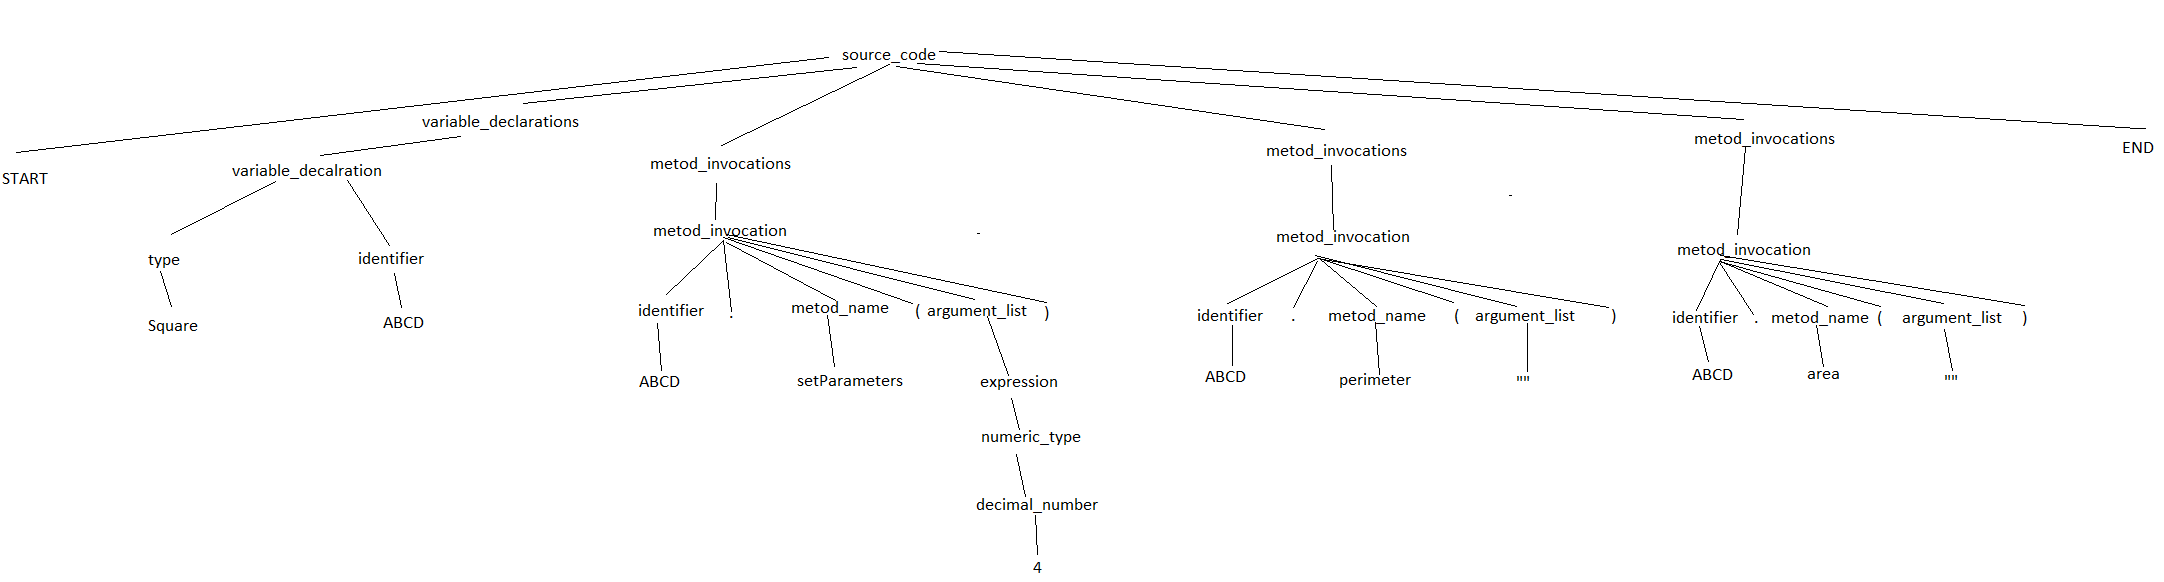
\includegraphics[width=\textwidth]{images/parse_tree.png} }

START

Square ABCD

ABCD.setParameters (4)

ABCD.perimeter()

ABCD.area()

END


